%=======================================================================
% riscv-trace.tex
%-----------------------------------------------------------------------

\documentclass[twoside,11pt]{book}
\usepackage{footnote}

\makesavenoteenv{tabulary}
\setcounter{tocdepth}{4}
\setcounter{secnumdepth}{4}

% Fix copy/pasting of ligatures in Acrobat
\input{glyphtounicode.tex}
\pdfgentounicode=1 %

% Package includes

\usepackage[T1]{fontenc}
\usepackage{textcomp}
\usepackage{lmodern}
\usepackage{graphicx}
\usepackage{geometry}
\usepackage{array}
\usepackage{colortbl}
\usepackage[colorlinks=true,linkcolor=blue]{hyperref}
\usepackage{placeins}
\usepackage{bbding}
\usepackage{longtable}
\usepackage{multirow}
\usepackage{float}
\usepackage{pdfpages}
\usepackage{placeins}
\usepackage{tabulary}
%\usepackage{listings}
\usepackage{algorithmicx}
\usepackage{program}
\usepackage[nochapter]{vhistory}
%\usepackage{tablefootnote}

% If LaTeX just doesn't do what I want, buy http://www.amazon.com/gp/product/0201362996

% Used for tables that can span pages:
\usepackage{xtab}

% Keep spacing normal in enumerated instead of adding extra space between
% items.
\usepackage{enumitem}
%\setlist{nolistsep}

\newenvironment{steps}[1]
  {
     \vspace{1ex}
     \noindent
     #1
     \begin{enumerate}
  }
  {
     \end{enumerate}
     \vspace{1ex}
 }

% Setup margins

\setlength{\topmargin}{-0.5in}
\setlength{\textheight}{9in}
\setlength{\oddsidemargin}{0in}
\setlength{\evensidemargin}{0in}
\setlength{\textwidth}{6.5in}

% Useful macros

\newcommand{\note}[1]{{\bf [ NOTE: #1 ]}}
\newcommand{\fixme}[1]{{\bf [ FIXME: #1 ]}}
\newcommand{\todo}[1]{\marginpar{\footnotesize #1}}

\newcommand{\wunits}[2]{\mbox{#1\,#2}}
\newcommand{\um}{\mbox{$\mu$m}}
\newcommand{\xum}[1]{\wunits{#1}{\um}}
\newcommand{\by}[2]{\mbox{#1$\times$#2}}
\newcommand{\byby}[3]{\mbox{#1$\times$#2$\times$#3}}

\newlength\savedwidth
\newcommand\whline[1]{%
  \noalign{%
    \global\savedwidth\arrayrulewidth\global\arrayrulewidth 1.5pt%
  }%
  \cline{#1}%
  \noalign{\vskip\arrayrulewidth}%
  \noalign{\global\arrayrulewidth\savedwidth}%
}

% Custom list environments

\newenvironment{tightlist}
{\begin{itemize}
 \setlength{\parsep}{0pt}
 \setlength{\itemsep}{-2pt}}
{\end{itemize}}

\newenvironment{titledtightlist}[1]
{\noindent
 ~~\textbf{#1}
 \begin{itemize}
 \setlength{\parsep}{0pt}
 \setlength{\itemsep}{-2pt}}
{\end{itemize}}

\newenvironment{commentary}
{ \vspace{-0.2in}
  \begin{quotation}
  \noindent
  \small \em
  \rule{\linewidth}{1pt}\\
}
{ 
  \end{quotation}
  \vspace{-0.2in}
}

% Other commands and parameters

\pagestyle{myheadings}
\setlength{\parindent}{0in}
\setlength{\parskip}{10pt}
\sloppy

% Commands for register format figures.

% New column types to use in tabular environment for instruction formats.
% Allocate 0.18in per bit.
\newcolumntype{I}{>{\centering\arraybackslash}p{0.18in}}
% Two-bit centered column.
\newcolumntype{W}{>{\centering\arraybackslash}p{0.36in}}
% Three-bit centered column.
\newcolumntype{F}{>{\centering\arraybackslash}p{0.54in}}
% Four-bit centered column.
\newcolumntype{Y}{>{\centering\arraybackslash}p{0.72in}}
% Five-bit centered column.
\newcolumntype{R}{>{\centering\arraybackslash}p{0.9in}}
% Six-bit centered column.
\newcolumntype{S}{>{\centering\arraybackslash}p{1.08in}}
% Seven-bit centered column.
\newcolumntype{O}{>{\centering\arraybackslash}p{1.26in}}
% Eight-bit centered column.
\newcolumntype{E}{>{\centering\arraybackslash}p{1.44in}}
% Ten-bit centered column.
\newcolumntype{T}{>{\centering\arraybackslash}p{1.8in}}
% Twelve-bit centered column.
\newcolumntype{M}{>{\centering\arraybackslash}p{2.2in}}
% Sixteen-bit centered column.
\newcolumntype{K}{>{\centering\arraybackslash}p{2.88in}}
% Twenty-bit centered column.
\newcolumntype{U}{>{\centering\arraybackslash}p{3.6in}}
% Twenty-bit centered column.
\newcolumntype{L}{>{\centering\arraybackslash}p{3.6in}}
% Twenty-five-bit centered column.
\newcolumntype{J}{>{\centering\arraybackslash}p{4.5in}}

\newcommand{\instbit}[1]{\mbox{\scriptsize #1}}
\newcommand{\instbitrange}[2]{~\instbit{#1} \hfill \instbit{#2}~}
\newcommand{\reglabel}[1]{\hfill {\tt #1}\hfill\ }

\newcommand{\wiri}{\textbf{WIRI}}
\newcommand{\wpri}{\textbf{WPRI}}
\newcommand{\wlrl}{\textbf{WLRL}}
\newcommand{\warl}{\textbf{WARL}}





% All registers are named here. That way when we rename one we'll get errors if
% there are still references to the old name.

\usepackage{makeidx}
\makeindex

\usepackage{xspace}
\usepackage{placeins}

\newcommand{\versionnum}{0.025-DRAFT}

%%% This file is generated by Makefile.
%%% Do not edit this file!\n%%%
    \gdef\GITHash{263c6d1f96b123d89df4ac6c9d96fd4d02abee99}    \gdef\GITAbrHash{263c6d1}    \gdef\GITAuthorDate{Tue Oct 1 17:53:02 2019 +0100}    \gdef\GITAuthorName{IainCRobertson}

\begin{document}
\setcounter{footnote}{0}

\title{RISC-V Processor Trace\\
Version \versionnum\\
\GITHash
}
\author{Gajinder Panesar \textless gajinder.panesar@ultrasoc.com\textgreater, UltraSoC Technologies Ltd.}

\maketitle

\markboth{RISC-V Processor Trace Version \versionnum}
{RISC-V Processor Trace Version \versionnum}
\thispagestyle{empty}

\frontmatter

\tableofcontents
\listoffigures
\listoftables

\mainmatter

\chapter{Introduction}
\label{sec:intro}

In complex systems understanding program behavior is not easy.
Unsurprisingly in such systems, software sometimes does not behave as
expected. This may be due to a number of factors, for example,
interactions with other cores, software, peripherals, realtime
events, poor implementations or some combination of all of the above.

It is not always possible to use a debugger to observe behavior of a
running system as this is intrusive.  Providing visibility of program
execution is important.  This needs to be done without swamping the
system with vast amounts of data.

One method of achieving this is via a Processor Branch Trace.

This works by tracking execution from a known start address and sending
messages about the address deltas taken by the program. These deltas are
typically introduced by jump, call, return and branch type instructions,
although interrupts and exceptions are also types of deltas.

Conceptually, the system has one or more of the following fundamental components:

\begin{itemize}
  \item
    A core with an instruction trace interface that outputs all relevant
    information to successfully create a processor branch trace and more.
    This is a high bandwidth interface: in most implementations, it will supply
    a large amount of data (instruction address, instruction type, context information, ...)
    for each CPU execution clock cycle.
  \item
    A hardware encoder that takes in the CPU instruction trace and compresses
    it into lower bandwidth trace packets.
  \item
    A transmission channel to transmit or a memory to store these trace packets.
  \item
    A decoder, usually software on an external PC, that takes in the trace
    packets and, with knowledge of the program binary that's running on the
    originating CPU, reconstructs the program flow. This decoding step can
    be done off-line or in real-time while the CPU is executing.
\end{itemize}

In RISC-V, all instructions are executed unconditionally or at least
their execution can be determined based on the program binary. The
instructions between the deltas can all assumed to be executed
sequentially. Because of this, there is no need to report sequential 
instructions in the trace, only whether the branches were taken or not
and the address of taken indirect branches or jumps. If the program
counter is changed by an amount that cannot be determined from the
execution binary, the trace decoder needs to be given the destination
address (i.e. the address of the next valid instruction).  Examples of
this are indirect branches or jumps, where the next instruction
address is determined by the contents of a register rather than a
constant embedded in the source code.

Interrupts generally occur asynchronously to the program's execution
rather than intentionally as a result of a specific instruction or
event.  Exceptions can be thought of in the same way, even though they
can be typically linked back to a specific instruction address.  The
decoder generally does not know where an interrupt occurs in the
instruction sequence, so the trace encoder must report the address
where normal program flow ceased, as well as give an indication of the
asynchronous destination which may be as simple as reporting the
exception type.  When an interrupt or exception occurs, or the
processor is halted, the final instruction executed beforehand must be
included in the trace.

This document serves to specify the ingress port (the signals between
the RISC-V core and the encoder), compressed branch trace algorithm and
the packet format used to encapsulate the compressed branch trace
information.

\subsection{Nomenclature}

In the following sections items in \textbf{bold} are signals or
attributes within a packet.

Items in \textit {italics} refer to parameters either built into the
hardware or configurable hardware values.

An encoder is a piece of hardware that takes in RISC-V instruction data
on its ingress port and transforms it into trace packets.

A decoder is a piece of software that takes the trace packets emitted by the
encoder and reconstructs the execution flow of the code executed in the RISC-V core.

RISC-V has the following definitions:
\begin{itemize}
  \item
    \textbf{Exception}: an unusual condition occurring at run time associated with an instruction in the current RISC-V hart
  \item
    \textbf{Interrupt}: an external asynchronous event that may cause a RISC-V hart to experience an unexpected transfer of control
  \item
    \textbf{Trap}: the transfer of control to a trap handler caused by either an exception or an interrupt
\end{itemize}
So, not all exceptions and interrupts cause traps. Most notably, floating point exceptions and disabled interrupts do not trap.

If an exception or interrupt doesn't trap, the program counter does not
change. So, there is no need to trace all exceptions/interrupts, just
traps.

In this document, interrupts and exceptions are only traced when they cause traps to be taken.

\chapter{Branch Trace} \label{Branch Trace}


\section{Instruction Delta Tracing} \label{Delta Tracing}

Instruction delta tracing, also known as branch tracing, works by
tracking execution from a known start address by sending information
about the deltas taken by the program. Deltas are typically introduced
by jump, call, return and branch type instructions, although
interrupts and exceptions are also types of deltas.

The approach relies on
an offline copy of the program binary being available to the decoder, so it
is generally unsuitable for either dynamic (self-modifying) programs
or those where access to the program binary is prohibited.

While the program binary is sufficient, access to the assembly or
higher-level source code will improve the ability of the decoder to present
the decoded trace in the debugger by annotating the traced instructions with
source code line numbers and labels, variable names etc.

This approach can be extended to cope with small sections of
deterministically dynamic code by arranging for the decoder to request
instruction memory from the target. Memory lookups generally lead to a
prohibitive reduction in performance, although they are suitable for
examining modest jump tables, such as the exception/interrupt vector
pointers of an operating system which may be adjusted at boot up and
when services are registered.  Both static and dynamically linked
programs can be traced using this approach. Statically linked programs
are straightforward as they generally operate in a known address
space, often mapping directly to physical memory. Dynamically linked
programs require the debugger to keep track of memory allocation
operations using either trace or stop-mode debugging.

\section{Contents of an Instruction Delta Trace} \label{Trace Contents}

\subsection{Sequential Instructions} \label{Sequential Instructions}

For instruction set architectures such as RISC-V where all instructions are executed
unconditionally or at least their execution can be determined based on
the program binary, the instructions between the deltas are assumed to be
executed sequentially. Consequently, there is no need
to report them in the trace. The trace only needs to contain whether
branches were taken or not, the addresses of taken indirect jumps, or
other program counter discontinuities.

\subsection{Uninferable PC Discontinuities} \label{uninfpc}

An uninferable program counter discontinuity is a program counter change
that can not be inferred from the program binary alone. For these cases,
the instruction delta trace must include a destination address: the
address of the next valid instruction.

Examples of this are indirect jumps, where
the next instruction address is determined by the contents of a
register rather than a constant embedded in the program binary.

\subsection{Branches} \label{branches}

A branch is an instruction where a jump is conditional on the
value of a register or a flag. For a decoder to able to follow program flow,
the trace must include whether a branch was taken or not.

For a direct branch, where the destination address is a constant that
is encoded in the program binary, no further information is required.
Direct branches are the only type of branch that is supported by the
RISC-V ISA.

\subsection{Interrupts and Exceptions} \label{interruptsexceptions}

Interrupts are a different type of delta that generally occur
asynchronously to the program's execution rather than intentionally as
a result of a specific instruction or event. Exceptions can be thought
of in the same way, even though they can be typically linked back to a
specific instruction address.

The decoder generally does not know
where an interrupt occured in the instruction sequence, so the trace
must report the address where normal program flow ceased, as well as
give an indication of the asynchronous destination which may be as
simple as reporting the exception type.  When an interrupt or
exception occurs, or the processor is halted, the final instruction
executed beforehand must be traced.  Following this, for an interrupt
or exception, the next valid instruction address (the first of the
interrupt or exception handler) must be traced in order to instruct the
trace decoder to classify the instruction as an indirect jump even
if it is not.

\subsection{Synchronization} \label{synchronization}

In order to make the trace robust there need to be regular
synchronization points within the trace. Synchronization is made by
sending a full valued instruction address (and potentially a context
identifier). The decoder and debugger may also benefit from sending
the reason for synchronising. The frequency of synchronization is a
trade-off between robustness and trace bandwidth.

The instruction trace encoder needs to synchronise fully:

\begin{itemize}

\item After a reset.
  \item When tracing starts.
\item If the instruction is the first of an interrupt service routine or
exception handler (hardware context change).
\item After a prolonged period of time.
\end{itemize}

\section{Optional and run-time configurable modes} \label{optional}

An instruction trace encoder may support multiple tracing modes.
To ensure that the decoder treats the incoming packets
correctly, it needs to be informed of the current active configuration.
The configuration is reported by a packet that is issued by the encoder
whenever the encoder configuration is changed.

Here are common examples of such modes:

\begin{itemize}
  \item delta address mode:
    program counter discontinuities are encoded as differences instead of absolute address values.
  \item full address mode:
    program counter discontinuities are encoded as absolute address values.
  \item implicit exception mode:
    destination addresses of CPU exceptions are assumed to be known by the decoder, and thus not encoded
    in the trace.
  \item implicit return mode:
    the destination address of function call returns is derived from a call stack, and thus not encoded
    in the trace.
  \item branch prediction mode:
    branches that are predicted correctly by an encoder branch predictor (and an identical copy in the decoder)
    are not encoded as taken/non-taken, but as a more efficient branch count number.
\end{itemize}

Modes may have associated parameters; see Table~\ref{tab:parameters} for further details.

\subsection{Delta address mode} \label{sec:delta-address}

Related parameters: None

In delta address mode, non-sequential program counter changes
are encoded as the difference between the previous and the current
address. This kind of encoding require less bits than encoding the
full address, and thus results in higher compression ratios.

This is the default encoding mode.

\subsection{Full address mode} \label{sec:full-address}

Related parameters: None

In full address mode, all addresses in the trace are encoded as absolute addresses instead
of in differential form. This kind of encoding is always less efficient, but it can be a useful 
debugging aid for software decoder developers.

\subsection{Implicit exception mode} \label{sec:implicit-exception}

Related parameters: None

The RISC-V Privileged ISA specification stores exception handler base
addresses in the \textbf{\textit{utvec/stvec/mvec}} CSR registers.
In some RISC-V implementations, the lower address bits are stored in
the \textbf{\textit{ucause/scause/mcause}} CSR registers.

By default, both the vec and cause values are reported when an exception or interrupt occurs.

The implicit exception mode omits vec, the trap handler address, from the trace and
thus improves efficiency.

This mode can only be used if the decoder can infer the address of the trap handler
from just the exception cause.

\subsection{Implicit return mode} \label{sec:implicit-return}

Related parameters: \textit{call\_counter\_size\_p}, \textit{return\_stack\_size\_p}.

Although a function return is usually an indirect jump, well behaved programs return to the
point in the program from which the function was called using a standard calling convention.
For those programs, it is possible to determine the execution path without being explicitly notified
of the destination address of the return.  The implicit return mode can result in very
significant improvements in trace encoder efficiency.

Returns can only be treated as inferable if the associated call has already been reported in
an earlier packet.  The encoder must ensure that this is the case.  This can be accomplished
by utilizing a counter to keep track of the number of nested calls being traced.  The counter
increments on calls (but not tail calls), and decrements on returns (see Section~\ref{Jump Classes}
for definitions).  The counter will not over or underflow, and is reset to 0 whenever a
synchronization packet is sent.  Returns will be treated as inferable and will not generate a trace
packet if the count is non-zero (i.e. the associated call was already reported in an earlier packet).

Such a scheme is low cost, and will work as long as programs are "well behaved".  The encoder does not check that the
return address is actually that of the instruction following the associated call.  As such, any program that
modifies return addresses cannot be traced using this mode with this minimal implementation.

Alternatively, the encoder can maintain a stack of expected return addresses, and only treat a
return as inferable if the actual return address matches the prediction.  This is fully robust for all
programs, but is more expensive to implement.  In this case, if a return address does not match the prediction, 
it must be reported explicitly via a packet, along with the number of return addresses
currently on the stack.  This ensures that the decoder can determine which return is being reported. 

\subsection{Branch prediction mode} \label{sec:branch-prediction}

Related parameters: \textit{bpred\_size\_p}.

In a straightforward encoder, the outcome of each executed branch is stored in
a branch map: a bit vector in which the taken/non-taken status of each branch is stored in
chronological order.

While this encoding is efficient, at 1 bit per branch, there are some cases where this
can still result in a relatively large volume of trace packets.  For example:

\begin{itemize}
  \item Executing tight loops of straight-line code.  Each iteration of the loop will add a bit to the branch map;
  \item Sitting in an idle loop waiting for an interrupt.  This produces large amounts of trace when nothing of 
  any interest is actually happening!  
  \item Breakpoints, which in some implementations also spin in an idle loop.
\end{itemize}

A significant coding efficiency can be obtained by the addition of a branch predictor in the encoder. To keep
the encoder and decoder synchronized, a predictor with identical behavior will need to be modelled in the decoder
software.

The predictor shall comprise a lookup table of 2\textsuperscript{N} entries, where N is specified by a parameter.  
Each entry is indexed by bits N:1 of the instruction address (or N+1:2 if compressed instructions aren't supported), 
and each contains a 2-bit prediction state:
\begin{itemize}
  \item 00: predict 0, transition to 01 if prediction fails;
  \item 01: predict 0, transition to 00 if prediction succeeds, else 11;
  \item 11: predict 1, transition to 10 if prediction fails;
  \item 10: predict 1, transition to 11 if prediction succeeds, else 00.
\end{itemize}

Other predictors, such as the gShare predictor (see Hennessy \& Patterson), should be considered.  Some further
experimentation is needed to determine the benefits of different lookup table sizes and predictor algorithms.

The lookup table entries are initialized to 00 when a synchronization packet is sent.


\chapter{Hart to encoder interface} \label{Interface}

\section{Instruction Trace Interface requirements}\label{sec:InstructionInterfaceRequirements}

This section describes in general terms the information which must be
passed from the RISC-V hart to the trace encoder for the purposes of
Instruction Trace, and distinguishes between what is mandatory, and
what is optional.

The following information is mandatory:

\begin{itemize}
  \item The number of instructions that are being retired;
  \item Whether there has been an exception or interrupt, and if so the cause 
        (from the \textbf{\textit{ucause/scause/vscause/mcause}} CSR)
        and trap value (from the \textbf{\textit{utval/stval/vstval/mtval}} CSR).

The register set to output should be the set that is updated as a result of the exception (i.e. 
the set associated with the privilege level immediately following the exception);

  \item The current privilege level of the RISC-V hart;
  \item The \textit{instruction\_type} of retired instructions for:
    \begin{itemize}
      \item Jumps with a target that cannot be inferred from the source code;
      \item Taken and nontaken branches;
      \item Return from exception or interrupt (\textbf{\textit{*ret}} instructions).
    \end{itemize}
  \item The \textit{instruction\_address} for:
    \begin{itemize}
      \item Jumps with a target that \textit{cannot} be inferred from the source code;
      \item The instruction retired immediately after a jump with a target that \textit{cannot} be inferred 
        from the source code (also referred to as the target or destination of the jump);
      \item Taken and nontaken branches;
      \item The last instruction retired before an exception or interrupt;
      \item The first instruction retired following an exception or interrupt;
      \item The last instruction retired before a privilege change;
      \item The first instruction retired following a privilege change.
    \end{itemize}
\end{itemize}

The following information is optional:

\begin{itemize}
  \item Context or Time information:
    \begin{itemize}
      \item The context and/or hart ID and/or time;
      \item The type of action to take when context or time data changes.
    \end{itemize}
  \item The \textit{instruction\_type} of instructions for:
    \begin{itemize}
      \item Calls with a target that \textit{cannot} be inferred from the source code;
      \item Calls with a target that \textit{can} be inferred from the source code;
      \item Tail-calls with a target that \textit{cannot} be inferred from the source code;
      \item Tail-calls with a target that \textit{can} be inferred from the source code;
      \item Returns with a target that \textit{cannot} be inferred from the source code;
      \item Returns with a target that \textit{can} be inferred from the source code;
      \item Co-routine swap;
      \item Jumps which don't fit any of the above classifications with a target that \textit{cannot} be inferred from the source code;
      \item Jumps which don't fit any of the above classifications with a target that \textit{can} be inferred from the source code.
    \end{itemize}
  \item If context or time is supported then the \textit{instruction\_address} for:
    \begin{itemize}
      \item The last instruction retired before a context or a time change;
      \item The first instruction retired following a context or time change.
    \end{itemize}
  \item Whether jump targets are sequentially inferable or not.
\end{itemize}

The mandatory information is the bare-minimum required to implement the branch trace algorithm outlined in Chapter~\ref{Algorithm}.  
The optional information facilitates alternative or improved trace algorithms:

\begin{itemize}
  \item Implicit return mode (see Section~\ref{sec:implicit-return}) requires the encoder to keep track of the number of nested 
    function calls, and to do this it must be aware of all calls and returns regardless of whether the target can be inferred or not;
  \item A simpler algorithm useful for basic code profiling would only report function calls and returns, again 
    regardless of whether the target can be inferred or not;
  \item Branch prediction techniques can be used to further improve the encoder efficiency, particularly for loops 
    (see Section~\ref{sec:branch-prediction}).  This requires the encoder to be aware of the address of all branches, whether
    they are taken or not.
  \item Uninferable jumps can be treated as inferable (which don't need to be reported in the trace output) if both the jump 
    and the preceding instruction which loads the target into a register have been traced.
\end{itemize}

\subsection{Jump classification and target inference} \label{Jump Classes}

Jumps are classified as \textit{inferable}, or \textit{uninferable}.  An \textit{inferable} jump has a target which can be
deduced from the binary executable or representation thereof (e.g. ELF).  For the purposes of this specification, the following 
strict definition applies:

If the target of a jump is supplied via a constant embedded within the jump opcode, it is classified as \textit{inferable}.
Jumps which are not \textit{inferable} are by definition \textit{uninferable}.

However, there are some jump targets which can still be deduced from the binary executable by considering pairs of instructions
even though by the above definition they are classified as uninferable.  Specifically, jump targets that are supplied via

\begin{itemize}
  \item an \textbf{\textit{lui}} or \textbf{\textit{c.lui}} (a register which contains a constant), or
  \item an \textbf{\textit{auipc}} (a register which contains a constant offset from the PC).
\end{itemize}

Such jump targets are classified as \textit{sequentially inferable} if the pair of instructions are retired consecutively 
(i.e. the \textbf{\textit{auipc}}, \textbf{\textit{lui}} or \textbf{\textit{c.lui}} immediately precedes the jump).  Note:
the restriction that the instructions are retired consecutively is necessary in order to minimize the additional signalling
needed between the hart and the encoder, and should have a minimal impact on trace efficiency as it is anticipated that
consecutive execution will be the norm. Support for sequentially inferable jumps is optional.

Jumps may optionally be further classified according to the recommended calling convention:

\begin{itemize}
  \item \textit{Calls}: 
    \begin{itemize}
      \item \textbf{\textit{jal}} x1;
      \item \textbf{\textit{jal}} x5;
      \item \textbf{\textit{jalr}} x1, rs  where rs != x5;
      \item \textbf{\textit{jalr}} x5, rs  where rs != x1;
      \item \textbf{\textit{c.jalr}} rs1 where rs1 != x5;
      \item \textbf{\textit{c.jal}}.
    \end{itemize}
  \item \textit{Tail-calls}: 
    \begin{itemize}
      \item \textbf{\textit{jal}} x0;
      \item \textbf{\textit{c.j}};
      \item \textbf{\textit{jalr}} x0, rs where rs != x1 and rs != x5;
      \item \textbf{\textit{c.jr}} rs1 where rs1 != x1 and rs1 != x5.
    \end{itemize}
  \item \textit{Returns}: 
    \begin{itemize}
      \item \textbf{\textit{jalr}} rd, rs where (rs == x1 or rs == x5) and rd != x1 and rd != x5;
      \item \textbf{\textit{c.jr}} rs1 where rs1 == x1 or rs1 == x5.
    \end{itemize}
  \item \textit{Co-routine swap}: 
    \begin{itemize}
      \item \textbf{\textit{jalr}} x1, x5;
      \item \textbf{\textit{jalr}} x5, x1;
      \item \textbf{\textit{c.jalr}} x5.
    \end{itemize}
  \item \textit{Other}: 
    \begin{itemize}
      \item \textbf{\textit{jal}} rd where rd != x1 and rd != x5;
      \item \textbf{\textit{jalr}} rd, rs where rs != x1 and rs != x5 and rd != x0 and rd != x1 and rd != x5.
    \end{itemize}
\end{itemize}

\subsection{Relationship between RISC-V core and the encoder} \label{sec:relationship}

The encoder is intended to encode the instructions executed on a single hart.  

It is however commonplace for a RISC-V core to contain multiple harts.  This can be 
supported by the core in several different ways:

\begin{itemize}
  \item Implement a separate instance of the interface per hart.  Each instance can be connected
    to a separate encoder instance, allowing all harts to be traced concurrently.  Alternatively,
    external muxing may be used in conjunction with a single encoder in order to trace one particular 
    hart at a time;
  \item Implement a singe interface for the core, with muxing inside the core to select which hart to 
  connect to the interface.
\end{itemize}

(Whilst it is technically feasible to use a single encoder with multiple harts operating 
in a fine-grained multi-threaded configuration, the frequent context changes that would occur
as a result of thread-switching would result in extremely poor encoding efficiency, and so
this configuration is not recommended.)

\section{Instruction Trace Interface}\label{sec:InstructionTraceInterface}
This section describes the interface between a RISC-V hart and the
trace encoder that conveys the information described in the section ~\ref{sec:InstructionInterfaceRequirements}.  
Signals are assigned to one of the  following groups:

\begin{itemize}
  \item M: Mandatory.  The interface must include an instance of this signal.
  \item O: Optional.  The interface may include an instance of this signal.
  \item MR: Mandatory, may be replicated. For harts that can retire a maximum of N "special" instructions per clock
    cycle, the interface must include N instances of this signal.
  \item OR: Optional, may be replicated. For harts that can retire a maximum of N "special" per clock
    cycle, the interface must include zero or N instances of this signal.
  \item BR: Block, may be replicated.  Mandatory for harts that can retire multiple instructions in a block.  
    Replication as per OR.  If omitted, the interface must include SR group signals instead.
  \item SR: Single, may be replicated.  Mandatory for harts that can only retire one instruction in a block.  
    Replication as per OR (see section~\ref{sec:alt-multi}).  If omitted, the interface must include BR 
    group signals instead.
\end{itemize}
"Special" instructions are those that require \textbf{itype} to be non-zero.

\begin{table}[htp]
    \centering
    \caption{Instruction interface signals}
    \label{tab:common-ingress}
    \begin{tabulary}{\textwidth}{|l|l|p{80mm}|}
        \hline
        \textbf{Signal} & \textbf{Group} & \textbf{Function} \\
        \hline
        \textbf{itype}[\textit{itype\_width\_p}-1:0] & MR & Termination type of the instruction block.  Encoding given in Table~\ref{tab:itype}
         (see Section~\ref{Jump Classes} for definitions of codes 6 - 15).\\
        \hline
        \textbf{cause}[\textit{ecause\_width\_p}-1:0] & M & Exception or interrupt cause (\textbf{\textit{ucause/scause/ vscause/mcause}}).
        Ignored unless \textbf {itype}=1 or 2.\\
        \hline
        \textbf{tval}[\textit{iaddress\_width\_p}-1:0] & M & The associated trap value, e.g. the
        faulting virtual address for address exceptions, as would be
        written to the \textbf{utval/stval/vstval/mtval} CSR. Future optional extensions may define \textbf{tval} 
        to provide ancillary information in cases where it currently supplies zero.
        Ignored unless \textbf{itype}=1 or 2.\\
        \hline
        \textbf{priv}[\textit{privilege\_width\_p}-1:0] & M & Privilege level for all instructions retired on this cycle.
        Encoding given in Table~\ref{tab:priv}.  Codes 4-7 optional.\\
        \hline
        \textbf{iaddr}[\textit{iaddress\_width\_p}-1:0] & MR & The address of the 1st instruction retired in this block.
        Invalid if \textbf{iretire}=0 \\
        \hline
        \textbf{context}[\textit{context\_width\_p}-1:0] & O & Context for all instructions retired on this cycle.\\
        \hline
        \textbf{time}[\textit{time\_width\_p}-1:0] & O & Time generated by the core.\\
        \hline
        \textbf{ctype}[\textit{ctype\_width\_p}-1:0] & O & Reporting behavior for \textbf{context}.  
        Encoding given in Table~\ref{tab:context-type}.  Codes 2-3 optional.\\
        \hline
        \textbf{sijump} & OR & If \textbf{itype} indicates that this block ends with an uninferable discontinuity, setting this signal to 1 
        indicates that it is sequentially inferable and may be treated as inferable by the encoder if the preceding 
        \textbf{\textit{auipc}}, \textbf{\textit{lui}} or \textbf{\textit{c.lui}} has been traced.  
        Ignored for \textbf{itype} codes other than 6, 8, 10, 12 or 14.\\
        \hline
    \end{tabulary}
\end{table}

\begin{table}[htp]
    \centering
    \caption{Instruction interface signals - multiple retirement per block}
    \label{tab:multi-ingress}
    \begin{tabulary}{\textwidth}{|l|l|p{80mm}|}
        \hline
        \textbf{Signal} & \textbf{Group} & \textbf{Function} \\
        \hline
        \textbf{iretire}[\textit{iretire\_width\_p}-1:0] & BR & Number of halfwords represented by instructions retired in this block.\\
        \hline
        \textbf{ilastsize}[\textit{ilastsize\_width\_p}-1:0] & BR & The size of the last retired instruction is 2\textsuperscript{\textbf{ilastsize}} half-words.\\
        \hline
    \end{tabulary}
\end{table}

\begin{table}[htp]
    \centering
    \caption{Instruction interface signals - single retirement per block}
    \label{tab:single-ingress}
    \begin{tabulary}{\textwidth}{|l|l|p{80mm}|}
        \hline
        \textbf{Signal} & \textbf{Group} & \textbf{Function} \\
        \hline
        \textbf{iretire}[0:0] & SR & Number of instructions retired in this block (0 or 1).\\
        \hline
        \textbf{ilastsize}[\textit{ilastsize\_width\_p-1}:0] & SR & The size of the retired instruction is 2\textsuperscript{\textbf{ilastsize}} half-words.\\
        \hline
    \end{tabulary}
\end{table}

\begin{table}[htp]
    \centering
    \caption{Instruction Type (\textbf{itype}) encoding}
    \label{tab:itype}
    \begin{tabulary}{\textwidth}{|l|p{140mm}|}
      \hline
      \textbf{Value} & \textbf{Description} \\
      \hline
      0  & Final instruction in the block is none of the other named \textbf{itype} codes\\
      1  & Exception. An exception that traps occurred following the final retired instruction in the block\\
      2  & Interrupt. An interrupt that traps occurred following the final retired instruction in the block\\
      3  & Exception or interrupt return\\
      4  & Nontaken branch\\
      5  & Taken branch\\
      6  & Uninferable jump if \textit{itype\_width\_p} is 3, reserved otherwise\\
      7  & reserved\\
      8  & Uninferable call\\
      9  & Inferrable call\\
      10 & Uninferable tail-call\\
      11 & Inferrable tail-call\\
      12 & Co-routine swap\\
      13 & Return\\
      14 & Other uninferable jump\\
      15 & Other inferable jump\\
      \hline
    \end{tabulary}
\end{table}

\begin{table}[htp]
    \centering
    \caption{Privilege level (\textbf{priv}) encoding}
    \label{tab:priv}
    \begin{tabulary}{\textwidth}{|l|p{140mm}|}
      \hline
      \textbf{Value} & \textbf{Description} \\
      \hline
        0 & U\\
        1 & S/HS\\
        2 & reserved\\
        3 & M\\
        4 & D (debug mode)\\
        5 & VU\\
        6 & VS\\
        7 & reserved\\
      \hline
    \end{tabulary}
\end{table}

Tables~\ref{tab:common-ingress} and ~\ref{tab:multi-ingress}
list the signals in the interface designed to efficiently support retirement of multiple 
instructions per cycle.  The following discussion describes the multiple-retirement behavior.  
However, for harts that can only retire one instruction at a time, the signalling can be 
simplified, and this is discussed subsequently in Section~\ref{sec:single-retire}.  

The information presented in a block represents a contiguous
block of instructions starting at \textbf{iaddr}, all of which retired
in the same cycle. Note if \textbf{itype} is 1 or 2 (indicating an
exception or an interrupt), the number of instructions retired may be
zero. \textbf{cause} and \textbf{tval} are only defined if
\textbf{itype} is 1 or 2. If \textbf{iretire}=0 and \textbf{itype}=0,
the values of all other signals are undefined.

\textbf{iretire} contains the number of (16-bit) half-words represented by
instructions retired in this block, and \textbf{ilastsize} the size of the last
instruction.  Half-words rather than instruction count enables the encoder to easily compute the address of
the last instruction in the block without having access to the size of every 
instruction in the block.  

\textbf{itype} can be 3 or 4 bits wide.  If \textit{itype\_width\_p} is 3, a single code (6) is used to 
indicate all uninferable jumps.  This is simpler to implement, but precludes use of the implicit return mode
(see section~\ref{sec:implicit-return}), which requires jump types to be fully classified.

Whilst \textbf{iaddr} is typically a virtual address, it does not affect the encoder's behavior
if it is a physical address.

For harts that can retire a maximum of N non-zero \textbf{itype} values per clock
cycle, the signal groups MR, OR and either BR or SR must be replicated N times.  
Typically N is determined by the maximum number of branches that can be retired per clock cycle.
Signal group 0 represents information about the oldest instruction block, and group N-1
represents the newest instruction block. The interface supports no more
than one privilege change, context change, 
exception or interrupt per cycle and so signals in
groups M and O are not replicated. Furthermore, \textbf{itype} can only
take the value 1 or 2 in one of the signal groups, and this must be
the newest valid group (i.e. \textbf{iretire} and \textbf{itype} must
be zero for higher numbered groups). If fewer than N groups are required 
in a cycle, then lower numbered groups must be used
first. For example, if there is one branch, use only group 0, if
there are two branches, instructions up to the 1st branch
must be reported in group 0 and instructions up to the 2nd branch
must be reported in group 1 and so on.

\textbf{sijump} is optional and may be omitted if the hart does not implement the logic to detect
sequentially inferable jumps.  If the encoder offers an \textbf{sijump} input it must also provide a
parameter to indicate whether the input is connected to a hart that implements this capability, or
tied off.  This is to ensure the decoder can be made aware of the hart's capability.  Enabling 
sequentially inferable jump mode in the encoder and decoder when the hart does not support it will
prevent correct reconstruction by the decoder. 

The \textbf{context} and/or the \textbf{time} field can be used to convey any additional information to the decoder.  For example:

\begin{itemize}
  \item The address space and virtual machine IDs (\textbf{ASID} and \textbf{VMID}
  respectively).  Where present it is recommended these values be wired to bits [15:0] and [29:16];
  \item The software thread ID;
  \item The process ID from an operating system;
  \item It could be used to convey the values of CSRs to the decoder by setting \textbf{context} to the 
    CSR number and value when a CSR is written;
  \item In cases where a single encoder is being shared amongst multiple harts 
  (see section~\ref{sec:relationship}), it could also be used to indicate the hart ID, in cases where the 
  hart ID can be changed dynamically.
\item Time from within the hart
\end{itemize}

Table~\ref{tab:context-type} specifies the actions for the various
\textbf{ctype} values.  A typical behavior would be for this signal to
remain zero except on the 1st retirement after a context change
or when a time value should be reported.
\textit{ctype\_width\_p} may be 1 or 2.  The reduced width option only
provides support for reporting context changes imprecisely.

\begin{table}[htp]
    \centering
    \caption{Context type \textbf{ctype} values and corresponding actions}
    \label{tab:context-type}
    \begin{tabulary}{\textwidth}{|l|l|p{90mm}|}
        \hline
        \textbf{Type} & \textbf{Value} & \textbf{Actions} \\
        \hline
        Unreported & 0 & No action (don't report context).\\
        \hline
        Report context imprecisely & 1 & An example would be a SW thread or operating system process change.\newline
        Report the new context value at the earliest convenient opportunity.\newline
        It is reported without any address information, and the assumption is that the precise 
        point of context change can be deduced from the source code (e.g. a CSR write). \\
        \hline
        Report context precisely  & 2 & Report the address of the 1st instruction retired in this block, and the new context.\newline
        If there were unreported branches beforehand, these need to be reported first.\newline
        Treated the same as a privilege change.\\
        \hline
        Report context as an & 3 &  An example would be a change of hart.\\
        asynchronous discontinuity & & 
        Need to report the last instruction retired on the previous context, as well as the 1st on the new context.\newline
        Treated the same as an exception.\\
        \hline
    \end{tabulary}
\end{table}

\subsection{Simplifications for single-retirement} \label{sec:single-retire}

For harts that can only retire one instruction at a time, the interface can be simplified to
the signals listed in tables~\ref{tab:common-ingress} and ~\ref{tab:single-ingress}.  The 
simplifications can be summarized as follows:
 
\begin{itemize}
  \item \textbf{iretire} simply indicates whether an instruction retired or not;
\end{itemize}

\textbf{Note:} \textbf{ilastsize} is still needed in order to determine the address of the next 
instruction, as this is the predicted return address for implicit return mode 
(see Section~\ref{sec:implicit-return}).

The parameter \textit{retires\_p} which indicates to the encoder the maximum number of 
instructions that can be retired per cycle can be used by an encoder capable of supporting single or 
multiple retirement to select the appropriate interpretation of \textbf{iretire}.  


\subsection{Alternative multiple-retirement interface configurations} \label{sec:alt-multi}

For a hart that can retire multiple instructions per cycle, but no more than one branch, the preferred 
solution is to use one instance of signals from groups BR, MR and OR.  However, if the hart can retire 
N branches in a cycle, N instances of signals from groups MR, OR and either SR or BR must be used 
(each instance can be either a single instruction or a block).

If the hart can retire N instructions per cycle, but only one branch, it is allowed (though not recommended)
to provide explicit details of every instruction retired by using N instances of signals from groups
SR, MR and OR.

\subsection{Optional sideband signals}

Optional sideband signals may be included to provide additional functionality, as described in
tables \ref{tab:ingress-side-band} and \ref{tab:egress-side-band}.

Note, any user defined information that needs to be output by the encoder
will need to be applied via the \textbf{context} input.

\begin{table}[htp]
    \centering
    \caption{Optional sideband encoder input signals}
    \label{tab:ingress-side-band}
    \begin{tabulary}{\textwidth}{|l|l|p{90mm}|}
        \hline
        \textbf{Signal} & \textbf{Group} & \textbf{Function} \\
        \hline
        \textbf{impdef}[\textit{impdef\_width\_p}-1:0] & O &  Implementation defined sideband signals.  A typical use for
        these would be for filtering (see Chapter~\ref{ch:filtering}.\\
        \hline
        \textbf{trigger}[2:0] & OR & A pulse on bit 0 will cause the encoder to start tracing, and continue until further 
        notice, subject to other filtering criteria also being met.\newline
        A pulse on bit 1 will cause the encoder to stop tracing until further notice.  See section~\ref{sec:trigger}).\\
        \hline
        \textbf{halted} & O & Hart is halted.  Upon assertion, the encoder will output a packet to report the address 
        of the last instruction retired before halting, followed by a support packet to indicate that tracing has stopped. 
        Upon deassertion, the encoder will start tracing again, commencing with a synchronization packet.
        \textbf{Note:} If this signal is not provided, it is strongly recommended that Debug mode can be signalled via a 3-bit 
          \textbf{privilege} signal.  This will allow tracing in Debug mode to be controlled via the optional filtering capabilities.\\
        \hline
        \textbf{reset} & O & Hart is in reset.  Provided the encoder is in a different reset domain to the hart, this
        allows the encoder to indicate that tracing has ended on entry to reset, and restarted on exit.  
        Behavior is as described above for halt.\\
        \hline
    \end{tabulary}
\end{table}

\begin{table}[htp]
    \centering
    \caption{Optional sideband encoder output signals}
    \label{tab:egress-side-band}
    \begin{tabulary}{\textwidth}{|l|l|p{125mm}|}
        \hline
        \textbf{Signal} & \textbf{Group} & \textbf{Function} \\
        \hline
        \textbf{stall} & O & Stall request to hart.  Some applications may require lossless trace, which can be achieved by
        using this signal to stall the hart if the trace encoder is unable to output a trace packet (for example due to 
        back-pressure from the packet transport infrastructure).\\
        \hline
    \end{tabulary}
\end{table}

\FloatBarrier
\subsection{Using trigger outputs from the Debug Module} \label{sec:trigger}

The debug module of the RISC-V hart may have a trigger unit. This defines a match control register
(\textbf{\textit{mcontrol}}) containing a 4-bit \textbf{action} field, and reserves codes 2 - 5 
of this field for trace use.  
These action codes are hereby defined as shown in table \ref{tab:debugModuleTriggerSupport}.
If implemented, each action must generate a pulse on an output from the hart, on the same cycle as the instruction which
caused the trigger is retired.  

\begin{table}[!h]
    \centering
    \caption{Debug Module trigger support (\textbf{\textit{mcontrol}} \textbf{action})}
    \label{tab:debugModuleTriggerSupport}
    \begin{tabulary}{\textwidth}{|l|p{140mm}|}
        \hline
        \textbf {Value} & \textbf {Description} \\
        \hline
        2 & \textit{Trace-on}.  This should be connected to 
        \textbf{trigger[0]} if the encoder provides it. \\ 
        \hline
        3 & \textit{Trace-off}.  This should be connected to 
        \textbf{trigger[1]} if the encoder provides it. \\
        \hline
        4 & \textit{Trace-notify}.  This should be connected to 
        \textbf{trigger[2]} if the encoder provides it. This will cause the encoder to output
        a packet containing the address of the last instruction in the block if it is enabled.\\
        \hline
    \end{tabulary}
\end{table}

Trace-on and Trace-off actions provide a means for the hart to control when tracing
starts and stops.  It is recommended that tracing starts from the oldest  
instruction retired in the cycle that Trace-on is asserted, and stops following the newest
instruction retired in the cycle that Trace-off is asserted (subject to any optional filtering).

Trace-notify provides means to ensure that a specified instruction is explicitly reported 
(subject to any optional filtering). This capability is sometimes known as a watchpoint.

\FloatBarrier
\subsection{Example retirement sequences}

\begin{table}[htp]
    \centering
    \caption{Example 1 : 9 Instructions retired over four cycles, 2 branches} 
    \label{tab:signal-block-9-instructions-2-branches}
    \begin{tabulary}{\textwidth}{|l|l|}
        \hline
        \textbf {Retired} & \textbf {Instruction Trace Block} \\
        \hline
        1000: \textbf{\textit{divuw}} &  \textbf{iretire}=7, \textbf{iaddr}=0x1000, \textbf{itype}=8\\
        1004: \textbf{\textit{add}} &  \\
        1008: \textbf{\textit{or}} &  \\
        100C: \textbf{\textit{c.jalr}} &  \\
        \hline
        0940: \textbf{\textit{addi}} &  \textbf{iretire}=3, \textbf{iaddr}=0x0940, \textbf{itype}=4\\
        0944: \textbf{\textit{c.beq}} &  \\
        \hline
        0946: \textbf{\textit{c.bnez}} &  \textbf{iretire}=1, \textbf{iaddr}=0x0946, \textbf{itype}=5\\
        \hline
        0988: \textbf{\textit{lbu}} &  \textbf{iretire}=4, \textbf{iaddr}=0x0988, \textbf{itype}=0\\
        098C: \textbf{\textit{csrrw}} &  \\
        \hline
    \end{tabulary}
\end{table}

\section{Data Trace Interface requirements}\label{sec:DataInterfaceRequirements}

This section describes in general terms the information which must be
passed from the RISC-V hart to the trace encoder for the purposes of
Data Trace, and distinguishes between what is mandatory, and what is
optional.

If Data Trace is not needed in a system then there is no requirement
for the RISC-V hart to supply any of the signals in section
~\ref{sec:DataTraceInterface}.

Data trace supports up to four data access types: load, store, atomic and CSR.  
Support for both atomic and CSR accesses are independently optional.

The signalling protocol can take one of two forms, depending on the needs of the RISC-V 
hart: \textit{unified} or \textit{split}.

Unified is the simplest form, suitable for simpler, in-order harts.  In this form, all
information about a data access is signalled by the RISC-V hart in the
same cycle that the associated data access instruction is reported on the instruction
trace interface.  

For harts with out of order or speculative execution capabilities, many loads may be in 
progress simultaneously, and this approach is not practical as it would require the hart 
to maintain a large amount of state relating to all the in-progress loads.  For this 
reason, the interface also supports splitting loads into two parts:

\begin{itemize}
  \item The \textit{request} phase provides all the information about the load that
    originates from the hart (address, size, etc.) when the instruction retires;
  \item The \textit{response} phase provides the data and response status when it has
    been returned to the hart from the memory system.
\end{itemize}

The two parts of a split load are associated by use of a transaction ID.

The code size working group is proposing push and pop instructions,
which will each potentially result in multiple loads or stores.  In this case, the 
resulting loads and stores must be reported individually on the interface.  If an exception
occurs part way through the sequence of loads or stores initiated by such an instruction,
and the instruction is re-executed after the exception handler has been serviced, the
load or store sequence must recommence from the beginning.

\section{Data Trace Interface}\label{sec:DataTraceInterface}

This section describes the interface between a RISC-V hart and the
trace encoder that conveys the information described in the
section~\ref{sec:DataInterfaceRequirements}.  Signals are assigned to
one of the following groups:

\begin{itemize}
  \item M: Mandatory.  The interface must include an instance of this signal;
  \item U: Unified.  Mandatory for unified signalling;
  \item S: Split.  Mandatory for split load signalling;
  \item O: Optional.  The interface may include an instance of this signal.
\end{itemize}

\begin{table}[htp]
    \centering
    \caption{Data interface signals}
    \label{tab:data-ingress}
    \begin{tabulary}{\textwidth}{|l|l|p{80mm}|}
        \hline
        \textbf{Signal} & \textbf{Group} & \textbf{Function} \\
        \hline
        \textbf{dretire} & M & Data access retired (when high)\\
        \hline
        \textbf{dtype}[\textit{dtype\_width\_p}-1:0] & M & Data access type.  Encoding given in Table~\ref{tab:itype}\\
        \hline
        \textbf{daddr}[\textit{daddress\_width\_p}-1:0] & M & The data access address\\
        \hline
        \textbf{dsize}[\textit{dsize\_width\_p}-1:0] & M & The data access size is 2\textsuperscript{\textbf{dsize}} bytes\\
        \hline
        \textbf{data}[\textit{data\_width\_p}-1:0] & U & The data\\
        \hline
        \textbf{iaddr\_lsbs}[\textit{iaddr\_lsbs\_width\_p}-1:0] & O & LSBs of the data access instruction address.  Required if \textit{retires\_p} > 1\\
        \hline
        \textbf{dblock}[\textit{dblock\_width\_p}-1:0] & O & Instruction block in which the data access instruction is retired.  Required if there 
          are replicated instruction block signals\\
        \hline
        \textbf{lrid}[\textit{lrid\_width\_p}-1:0] & S & Load request ID. Valid when \textbf{dretire} is high\\
        \hline        
        \textbf{lresp}[\textit{lresp\_width\_p}-1:0] & S & Load response:\newline
        0: None\newline
        1: reserved\newline
        2: Okay.  Load successful; \textbf{ldata} valid\newline
        3: Error. Load failed; \textbf{ldata} not valid\\
        \hline        
        \textbf{lid}[\textit{lrid\_width\_p}-1:0] & S & Split Load ID. Valid when \textbf{lresp} is non-zero\\
        \hline        
        \textbf{sdata}[\textit{sdata\_width\_p}-1:0] & S & Store data. Valid when \textbf{dretire} is high\\
        \hline        
        \textbf{ldata}[\textit{ldata\_width\_p}-1:0] & S & Load data. Valid when \textbf{lresp} is non-zero\\
        \hline        
    \end{tabulary}
\end{table}

\begin{table}[htp]
    \centering
    \caption{Data access type (\textbf{dtype}) encoding}
    \label{tab:dtype}
    \begin{tabulary}{\textwidth}{|l|p{140mm}|}
      \hline
      \textbf{Value} & \textbf{Description} \\
        \hline
        0  & Load\\
        1  & Store\\
        2  & reserved\\
        3  & reserved\\
        4  & CSR read-write\\
        5  & CSR read-set\\
        6  & CSR read-clear\\
        7  & reserved\\
        8  & Atomic swap\\
        9  & Atomic add\\
        10 & Atomic AND\\
        11 & Atomic OR\\
        12 & Atomic XOR\\
        13 & Atomic max\\
        14 & Atomic min\\
        15 & Conditional store failure\\
      \hline
    \end{tabulary}
\end{table}

All signals in M, U and O groups are only valid when \textbf{dretire} is high.  Signals in the S group are valid as
indicated in table \ref{tab:data-ingress}.  

For harts that can retire a maximum of M data accesses per cycle, the implemented signal
groups must be replicated M times.  If fewer than M groups are required in a cycle, then lower numbered groups must 
be used first. For example, if there is one data access, use only group 0.

The maximum value of \textit{dtype\_width\_p} is 4.  However, if only loads and stores are supported, 
\textit{dtype\_width\_p} can be 1.  If CSRs are supported but atomics are not, \textit{dtype\_width\_p} can be 3.

Atomic and CSR accesses have either both load and store data, or store data and an operand.  For CSRs and unified
atomics, both values are reported via \textbf{data}, with the store data in the LSBs and the load data or operand
in the MSBs.

\textit{lrid\_width\_p} is determined by the maximum number of loads that can be in progress simultaneously, such
that at any one time there can be no more than one load in progress with a given ID.

\textbf{iaddr\_lsbs} and \textbf{dblock} are provided to support filtering of which data accesses to trace
based on their instruction address.  This is best illustrated by considering the following instruction sequence:

\begin{enumerate}
  \item load
  \item <some non data access instruction>
  \item load
  \item <some non data access instruction>
  \item <some non data access instruction>
\end{enumerate}
 
Suppose the hart is capable of retiring up to 4 instructions in a cycle, via a single block.   Instruction trace is 
enabled throughout, but the requirement is to collect data trace for the 1st load (instruction 1), and filtering is
configured to match the address of this instruction only.  However, information about instruction addresses is passed 
to the encoder at the block level, and the block boundaries are invisible to the decoder.  For instruction trace, 
all instructions in a block are traced if any of the instructions in that block match the filtering criteria.  
That is fine for instruction trace - the address of the 1st and last traced instruction are output explicitly.  
There will be some fuzziness about precisely what those addresses will be depending on where the block boundaries 
fall, but this is not a concern as everything is always self-consistent.
 
However, that is not the case for data trace.  Consider two scenarios:

\begin{itemize}
  \item Case 1: 1st block contains instructions 1, 2, 3; second block contains 4, 5
  \item Case 2: 1st block contains instructions 1,2; second block contains 3, 4, 5
\end{itemize}
 
Given that \textbf{dvalid} is high in the same cycle that the data access retires, the encoder knows the address of 
the 1st and last instructions in a block, but does not know precisely where in the block the data access is.  
In both cases, the first block matches the filtering criteria (it contains the address of instruction 1), and the second block does not.  
But if the encoder traced all the data accesses in the matching block, then in case 1 it would trace both instructions 1 and 3, whereas 
in the second case it would trace only instruction 1.  The decoder has no visibility of the block boundaries so cannot account for this.
It is expecting only instruction 1 to be traced, and so may misinterpret instruction 3.  If this code is in a loop for example, it will 
assume that the 2nd traced load is in fact instruction 1 from the next loop iteration, rather than instruction 3 from this iteration.
 
Providing the LSBs of the data access instruction address allows the decoder to determine precisely whether the data access should be 
traced or not, and removes the dependency on the block sizes and boundaries.  The number of bits required is one more bit than the 
number required to index within the block because blocks can start on any half-word boundary.
 
For harts that replicate the block signals to allow multiple blocks to retire per cycle it is also necessary to indicate which block 
each data access is associated with, so the encoder knows which block address to combine with the LSBs in order to construct the 
actual data access instruction address.  1 bit for 2 blocks per cycle, 2 bits for 4, and so on.


\chapter{Filtering} \label{ch:filtering}


The instruction trace encoder must be able to filter on the following inputs to the encoder:

\begin{itemize}
  \item The instruction address 
  \item The context 
  \item The exception cause 
  \item Whether the exception is an interrupt or not 
  \item The privilege level
  \item Tval 
  \item User specific signals
\end{itemize}

Internal to the encoder will be several comparators and filters. The
actual number of these will vary for different classes of devices. The
filters and comparators must be configured to provide the trace and
filtering required. There will be three command types needed to set up
the filtering operation.

\begin{enumerate}
    \item Set up comparator 
    \begin{itemize}
      \item Which input bus to compare
        \begin {enumerate}
          \item instruction
          \item address
          \item context
          \item tval
          \item exception
          \item user
        \end{enumerate}
      \item Value e.g. start address
    \end{itemize}
    \item Set up filter 
    \begin{itemize}
      \item Which comparator(s) to use which filtering operation to enable
        \begin {enumerate}
          \item \textit {eq}
          \item \textit {neq}
          \item \textit {lt}
          \item \textit {lte}
          \item \textit {gt}
          \item \textit {gte}
          \item \textit {always}
          \end{enumerate}
    \end{itemize}
    \item Set match 
    \begin{itemize}
      \item Configure matching behaviour for exception, privilege and user sideband
    \end{itemize}
\end{enumerate}

The user may wish to:

\begin{enumerate}
  \item Trace instructions between a range of addresses
  \item Trace instruction from one address to another
  \item Trace interrupt service routine
  \item Start/stop trace when in a particular privilege 
  \item Start/stop trace when context changes or is a particular value
  \begin {itemize}
    \item This can be HARTs and/or software contexts. If the latter this would be 
    \item Start/stop trace when specific instruction
    \item Start/stop using User specific signals 
    \item This could be the specific CSR value being presented to the Encoder
  \end{itemize}
\end{enumerate}

\chapter{Reference Compressed Branch Trace Algorithm} \label{Algorithm}

The contents of this chapter are informative only.

A reference algorithm for compressed branch trace is given in figure~\ref{fig:algo}.  
In the diagram, the following terms are used:

\begin{itemize}
  \item \textit{te\_inst.} The name of the packet type emitted by the encoder (see Chapter~\ref{packets});
  \item \textit{inst.}  Abbreviation for 'instruction';
  \item \textit{exception.  Exception or interrupt signalled;}
  \item \textit{updiscon.}  Uninferable PC discontinuity.  This identifies an instruction that
    causes the program counter to be changed by an amount that cannot be predicted from the
    source code alone (\textbf{itype} values 8, 10, 12 or 14);
  \item \textit{Qualified?}  An instruction that meets the filtering criteria is qualified, and will be traced;
  \item \textit{Branch?} Is the instruction a branch or not (\textbf{itype} values 4 or 5);
  \item \textit{branch map.}  A vector where each bit represents the outcome of a branch.  A 0 indicates the
    branch was taken, a 1 indicates that it was not;
  \item \textit{ppccd.} Privilege has changed, or context has changed and needs to be 
    reported precisely or treated as an uninferable PC discontinuity (see Table~\ref{tab:context-type});
  \item \textit{ppccd\_br.} As above, but branch map not empty;
  \item \textit{er\_n.}  Instruction retirement and exception signalled on the same cycle, or
    Trace-notify trigger (see Table~\ref{tab:debugModuleTriggerSupport});
  \item \textit{exc\_only.}  Exception or interrupt signalled without simultaneous retirement;
  \item \textit{cci.}  context change that can be reported imprecisely (see Table~\ref{tab:context-type});
  \item \textit{rpt\_br.} Report branches due to full branch map or misprediction;
  \item \textit{branches.}  The number of branches encountered but not yet reported to the decoder;
  \item \textit{pbc.} Correctly predicted branches count (always zero if branch predictor disabled or not present);
  \item \textcolor{cyan}{\textit{Reported?} Exception reported with \textbf{ehaddr} = 0 on the cycle it occured 
    because it was preceded by an updiscon;}
  \item \textit{resync count.} A counter used to keep track of when it is necessary to send 
    a synchronization packet (see Section~\ref{sec:resync});
  \item \textit{max\_resync.}  The resync counter value that schedules a synchronization packet (see Section~\ref{sec:resync});
  \item \textit{resync\_br.} The resync counter has reached the maximum value and there are
    entries in the branch map that have not yet been output (see Section~\ref{sec:resync}).
\end{itemize}

\begin{figure}
\begin{center}
  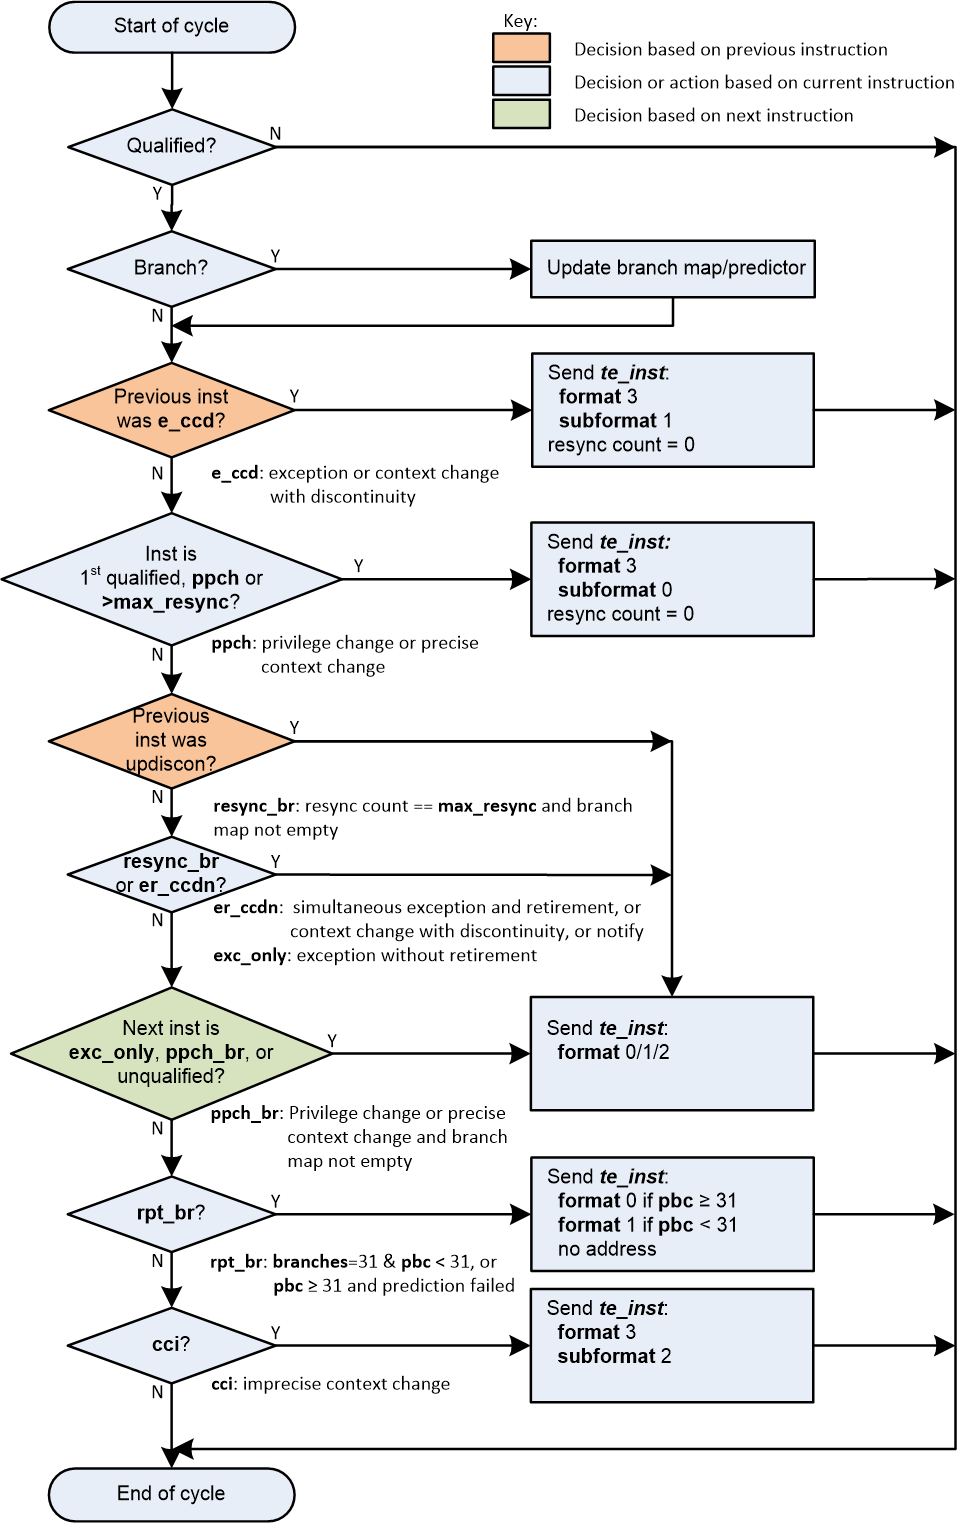
\includegraphics[height=23cm, width=15cm]{algo.png}
  \caption{Instruction delta trace algorithm}
  \label{fig:algo}
\end{center}
\end{figure}

Figure~\ref{fig:algo} shows instruction by instruction behavior, as would be
seen in a single-retirement system only.  Whilst the core to encoder interface allows the 
RISC-V hart to provide information on multiple retiring instructions simultaneously, the resultant 
packet sequence generated by the encoder must be the same as if retiring one instruction at a time.

A 3-stage pipeline within the encoder is assumed, such that the encoder has 
visibility of the current, previous and next instructions.  All packets are generated using 
information relating to the current instruction.  The orange diamonds indicate decisions 
based on the previous instruction, the green diamond indicates a decision based on the
next instruction, and all other diamonds are based on the current instruction.

Additionally, the encoder can generate one further packet type, not shown on the diagram for 
clarity.  The \textit{support} packet (format 3, subformat 3 - see section~\ref{sec:format33}) is 
sent when:

\begin{itemize}
  \item The encoder is enabled or disabled, or its configuration is changed, 
    to inform the decoder of the operating mode of the encoder;
  \item After the final qualified instruction has been traced, to inform the decoder that 
    tracing has stopped;
  \item If trace packets are lost (for example if the buffer into which packets are being 
    written fills up.  In this situation, the 1st packet 
    loaded into the buffer when space next becomes available must be a \textit{support} 
    packet.  Following this, tracing will resume with a sync packet.
\end{itemize}

Note: if the \textbf{halted} or \textbf{reset} sideband signals are asserted (see Table~\ref{tab:ingress-side-band})
the encoder will behave as if it has received an unqualified instruction (output \textit{te\_inst}
reporting the address of the previous instruction, followed by \textit{te\_support});


\section{Format selection} \label{format-selection}

In all cases but two, the packet format is determined only by a 'yes' outcome from the 
associated decision.  

When reporting branch information on its own (without an address), the choice between format 1 and format 0, 
subformat 0 depends on the number of correctly predicted branches (this will be 0 if the predictor is not 
supported, or is disabled).  No packets are generated until there are at least 31 branches to report.  
Format 1 is used if the outcome of at least one of those 31 branches was not predicted correctly.  If all were 
predicted correctly, nothing is output at this time, and the encoder continues to count correctly predicted
branch outcomes.  As soon as one of the branch outcomes is not correctly predicted, the encoder will output
a format 0, subformat 0 packet.  See also section~\ref{sec:format0}.

The choice between formats for the "format 0/1/2" case in the middle of the diagram also needs further 
explanation.  

\begin{itemize}
  \item If the number of correctly predicted branches is 31 or more, then format 0, subformat 0 is
    always used;
  \item Else, if the jump target cache is supported and enabled, and the address being reported is in the cache,
    then normally format 0, subformat 1 will be used, reporting the cache index associated with the address.  
    This will include branch information if there are any branches to report.  
    However, the encoder may chose to output the equivalent format 1 or 2 packet (containing the differential 
    address, with or without branch information) if that will result in a shorter packet 
    (see section~\ref{sec:format0});
  \item Else, if there are branches to report, format 1 is used, otherwise format 2.
\end{itemize}


Packet formats 0, 1 and 2 are organized so that the address is usually the final field.  Minimizing the 
number of bits required to represent the address reduces the total packet size and significantly
improves efficiency.  See Chapter~\ref{packets}.

\section{Resynchronisation} \label{sec:resync}

Per Section~\ref{synchronization}, a format 3 synchronisation packet must be output after "a prolonged
period of time". The exact mechanism for
determining this is not specified, but options might be to count the number of \textit{te\_inst} packets emitted, 
or the number of clock cycles elapsed, since the previous synchronization message was sent.

When the resync is required, the primary objective is to output a format 3 packet, so that the decoder can 
start tracing from that point without needing any of the history.  However, if the decoder is already synced, 
then it is also required that it can continue to follow the execution path up to and through the format 3 packet 
seamlessly.  As such, before outputting a format 3 packet, it is necessary to output a format 1 packet for the 
preceding instruction if there are any unreported branches (because format 3 does not contain a branch map).  
The format 3 will be sent if the resync timer has been exceeded.  On the cycle before this (when the resync timer 
value has been exactly reached), a format 1 will be generated if the branch map is not empty.

\section{Multiple retirement considerations} \label{rec:multiretcon}

As noted earlier in this section, for a single-retirement system the reference algorithm is applied to each retired
instruction.  When instructions are retired in blocks, only the first and last instruction in a block need be
considered, as all those in between are "uninteresting", and will have no effect on the encoder's state (their route
through figure~\ref{fig:algo} does not pass through any of the rectangular boxes).

In most cases, either the first or last instruction of a block (but not both) is interesting, meaning that the 
encoder does not need to generate more than one packet from a block.  However, there are a few cases where this
is not true, and it is possible that the encoder will need to generate two packets from the same block.  

For example, the first instruction in a block must generate a packet if it is the first traced instruction.  However,
if the block also indicates an exception or interrupt (\textbf{itype}= 1 or 2), then the last instruction in the block 
must also generate a packet.

As generating multiple packets per cycle would significatly complicate the encoder, and as situations such as this
will only occur infrequently, some elastic buffering in the encoder is the preferred approach.  This will allow subsequent
blocks to be queued whilst the encoder generates two successive packets from a block.  The encoder can drain the 
elastic buffer any time there is a cycle when the hart doesn't report anything, or if there is a block with 
\textbf{itype} = 0 (which is uninteresting to the encoder).

There are pathological cases where consecutive blocks could require packets to be generated from both first and last
instructions, but elastic buffering is only required if the blocks are also input on consecutive cycles.  In practice
there are very few cases where this can occur.  The worst so far identified case is a variation on the example above, 
where the exception is an ecall, and that in turn encounters some other form of exception or interrupt in the first 
few instructions of the trap handler:

\begin{itemize}
  \item Block 1: \textbf{itype} = 1 (ecall), \textbf{iretires} > 1.  Generate packet from first instruction (first traced),
    and last instruction (last before ecall);
  \item Block 2: \textbf{itype} = 1 or 2 (some other exception or interrupt), \textbf{iretires} > 0.  
    Generate packet from first instruction (ecall trap handler), and last instruction (last before other exception or interrupt);
  \item Block 3: Generate packet from first instruction (other exception or interrupt trap handler)
\end{itemize}

Because the ecall is known to the hart's fetch unit and can be predicted, it may be possible for block 2 to occur the cycle 
after block 1.  However, it is reasonable to assume that the other exception or interrupt will not be predictable, and as a result
there will be several cycles between blocks 2 and 3, which will allow the encoder to 'catch up'.  It is recommended that encoders
implement sufficient elastic buffering to handle this case, and if for some reason the elastic buffer overflows, it should
issue a support packet indicating trace lost.

\chapter{Trace Encoder Output Packets} \label{packets}

The bulk of this section describes the payload of packets output from the Trace Encoder.  
The infrastructure used to transport these packets is outside the scope of this document, and
as such the manner in which packets are encapsulated for transport is not specified.
However, the following information must be provided to the encapsulator:

\begin{itemize}
  \item The packet type;
  \item The packet length, in bytes;
  \item The packet payload.
\end{itemize}

Two example transport schemes are the UltraSoC Messaging Infrastructure, and the Arm Trace Bus.
Figure~\ref{fig:packet-format} shows the encapsulation used for the UltraSoC infrastructure:
\begin{itemize}
  \item The header byte contains a 5-bit field specifying the payload length in bytes, a 2-bit
    field indicating the "flow" (destination routing indicator), and a bit to indicate whether
    an optional 16-bit timestamp is present;
  \item The index field indicates the source of the packet.  The number of bits is system dependent,
    And the initial value emitted by the trace encoder is zero (it gets adjusted as it propagates 
    through the infrastructure);
  \item An optional 2-byte timestamp;
  \item The packet payload.
\end{itemize}

\begin{figure}[h]
  \begin{center}
    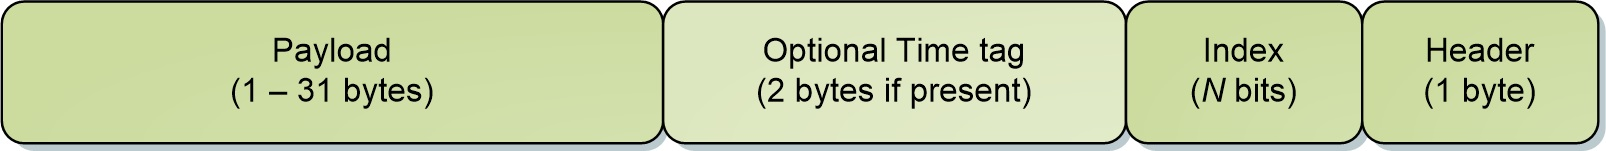
\includegraphics[height=1cm, width=9cm]{newPacket.jpg}
    \caption{Example Encapsulated Packet Format}
    \label{fig:packet-format}
  \end{center}
\end{figure}


Alternatively, for ATB, the source of the packet is indicated by the \textbf{ATID} bus field, and there is
no equivalent of "flow", so an example encapsulation might be:
\begin{itemize}
  \item A 5-bit field specifying the payload length in bytes
  \item A bit to indicate whether an optional 16-bit timestamp is present;
  \item An optional 2-byte timestamp;
  \item The packet payload.
\end{itemize}
It may be desirable for packets to start aligned to an ATB word, in which the \textbf{ATBYTES} bus field
in the last beat of a packet can be used to indicate the number of valid bytes.

The remainder of this section describes the contents of the payload
portion which should be independent of the infrastructure.  In each table, the fields are listed in
transmission order: first field in the table is transmitted first, and multi-bit fields are 
transmitted LSB first.

This packet payload format is used to output encoded instruction
trace.  Three different formats are used according to the needs of the
encoding algorithm. The following tables show the format of the
payload - i.e. excluding any encapsulation.

In order to achieve best performance, actual packet lengths may be adjusted using 'sign based compression'.
At the very minimum this should be applied to the address field of format 1 and 2 packets, but ideally will 
be applied to the whole packet, regardless of format.  This technique eliminates identical bits from the most 
significant end of the packet, and adjusts the length of the packet accordingly.  A decoder receiving this 
shortened packet can reconstruct the original full-length packet by sign-extending from the most significant
received bit.  An example of how this technique is used to choose between address formats is given in 
Section~\ref{addresses}.  The same principle can be applied to the entire packet, and the length (typically 
given in bytes) adjusted accordingly.

Where the payload length given in the following tables, or after applying sign-based compression, is not a 
multiple of whole bytes in length, the payload must be sign-extended to the nearest byte boundary.

Whilst offering maximum encoding efficiency, variable length packets can present some challenges,
specifically in terms of identifying where the boundaries between packets occur either when packed
packets are written to memory, or when packets are streamed offchip via a communications channel.  Two 
potential solutions to this are as follows:

\begin{itemize}
  \item If the maximum packet payload length is 2\textsuperscript{N}-1 (for example, if N is 5, then the maximum length is
    31 bytes), and the minimum packet payload length is 1, then a sequence of at least 2\textsuperscript{N} zero 
    bytes cannot occur within a packet payload, and therefore the first non-zero byte seen after a sequence of 
    at least 2\textsuperscript{N} zero bytes must be the first byte of a packet.  This approach can be used for
    alignment in either memory or a data stream;
  \item An alternative approach suitable for packets written to memory is to divide memory into blocks of M bytes
    (e.g. 1kbyte blocks), and write packets to memory such that the first byte in every block is always the first
    byte of a packet.  This means packets cannot span block boundaries, and so zero bytes must be used to pad between 
    the end of the last message in a block and the block boundary.
\end{itemize}

\begin{table}[htp]
  \centering
  \caption{Packet Payload Format 1 - with address}
  \label{tab:te_inst0-1-addr}
  \begin{tabulary}{\textwidth}{|l|p{35mm}|p{80mm}|}
    \hline
    {\bf Field name} & {\bf Bits} & {\bf Description} \\
    \hline
    \textbf{format}	& 2	& 01 (diff-delta): includes branch map and may include differential address\\
    \hline
    \textbf{branches} & 5 & Number of valid bits in branch-map. The length of branch-map is determined as follows: \newline
    0:      (cannot occur for this format) \newline
    1: 	1 bit \newline
    2-9: 	9 bits \newline
    10-17: 	17 bits \newline
    18-25: 	25 bits \newline
    26-31: 	31 bits \newline
    For example if branches = 12, the branch-map is 17 bits long, and the 12 LSBs are valid. \newline
    In most cases when the branch map is full there is no need to report an address,
    and this is indicated by setting branches to 0.  The exception to this is when 
    the instruction immediately prior to the final branch causes an uninferable discontinuity.\\
    \hline
    \textbf{branch\_map} & Determined by \newline 
                 \textbf{branches} field. & 
                 An array of bits indicating whether branches are taken or not.\newline
    Bit 0 represents the oldest branch instruction executed.   For each bit: \newline
    0: branch taken \newline
    1: branch not taken \\
    \hline
    \textbf{address}	& \textit {iaddress\_width\_p - iaddress\_lsb\_p} & 
                Differential instruction address.\\
    \hline
    \textbf{updiscon}	& 1 & 
                If the value of this bit is different from the MSB of \textbf{address}, it indicates that this 
                packet is reporting the instruction following an uninferable discontinuity and is also the 
                instruction before an exception, privilege change or resync 
                (i.e. it will be followed immediately by a format 3 \textit{te\_inst}).\\
    \hline
    \textbf{irfail}	& 1 & 
                If the value of this bit is different from \textbf{updiscon}, it indicates that this
                packet is reporting the instruction following a return because its address differs from 
                the predicted return address at the top of the implicit\_return return address stack.\\
    \hline
    \textbf{irdepth}	& \textit {call\_counter\_size\_p} & 
                If the value of \textbf{irfail} is different from \textbf{updiscon}, this field indicates 
                the number of entries on the return address stack (i.e. the entry number of the return that
                failed).  If \textbf{irfail} is the same value as \textbf{updiscon}, all bits in this field 
                will also be the same value as \textbf{updiscon}. \\
    \hline
  \end{tabulary}
\end{table}

\begin{table}[htp]
  \centering
  \caption{Packet Payload Format 1  - no address, branch map}
  \label{tab:te_inst0-1-noaddr-map}
  \begin{tabulary}{\textwidth}{|l|p{35mm}|p{80mm}|}
    \hline
    {\bf Field name} & {\bf Bits} & {\bf Description} \\
    \hline
    \textbf{format}	& 2	& 01 (diff-delta): includes branch map and may include differential address\\
    \hline
    \textbf{branches} & 5 & Number of valid bits in branch-map. The length of branch-map is determined as follows: \newline
    0:      31 bits, no \textbf{address} in packet \newline
    1-31: 	(cannot occur for this format) \\
    \hline
    \textbf{branch\_map} & 31 & 
                 An array of bits indicating whether branches are taken or not.\newline
    Bit 0 represents the oldest branch instruction executed.   For each bit: \newline
    0: branch taken \newline
    1: branch not taken \\
    \hline
    \textbf{branch\_fmt} & 2  & Both bits set to the same value as \textbf{branch\_map[MSB]} indicates that the
    preceding field is \textbf{branch\_map}. \\
    \hline
  \end{tabulary}
\end{table}

\begin{table}[htp]
  \centering
  \caption{Packet Payload Format 1 - no address, branch count}
  \label{tab:te_inst0-1-noaddr-count}
  \begin{tabulary}{\textwidth}{|l|p{35mm}|p{80mm}|}
    \hline
    {\bf Field name} & {\bf Bits} & {\bf Description} \\
    \hline
    \textbf{format}	& 2	& 01 (diff-delta): includes branch map and may include differential address\\
    \hline
    \textbf{branches} & 5 & Number of valid bits in branch-map. The length of branch-map is determined as follows: \newline
    0:      31 bits, no \textbf{address} in packet \newline
    31-1: 	(cannot occur for this format) \\
    \hline
    \textbf{branch\_count} & 16 & Count of the number of correctly predicted branches, minus 31. \\
    \hline
    reserved & 15 & zero\\
    \hline
    \textbf{branch\_fmt} & 2 & Set to 01, indicates that the packet contains a \textbf{branch\_count} field, no
    \textbf{address} field, and that the next branch failed prediction. \\
    \hline
  \end{tabulary}
\end{table}

\begin{table}[htp]
  \centering
  \caption{Packet Payload Format 1 - differential address, branch count}
  \label{tab:te_inst0-1-addr-count}
  \begin{tabulary}{\textwidth}{|l|p{35mm}|p{80mm}|}
    \hline
    {\bf Field name} & {\bf Bits} & {\bf Description} \\
    \hline
    \textbf{format}	& 2	& 01 (diff-delta): includes branch map and may include differential address\\
    \hline
    \textbf{branches} & 5 & Number of valid bits in branch-map. The length of branch-map is determined as follows: \newline
    0:      31 bits, no \textbf{address} in packet \newline
    31-1: 	(cannot occur for this format) \\
    \hline
    \textbf{branch\_count} & 16 & Count of the number of correctly predicted branches, minus 31. \\
    \hline
    \textbf{address (LSBs)}	& 15 & 
                15 LSBs of differential instruction address.\\
    \textbf{branch\_fmt} & 2 & Set to 10, indicates that the packet contains a \textbf{branch\_count} field and
     an \textbf{address} field. This will be the case if the packet is output because it is necessary to report an
     address (e.g. following an updiscon, or if the next instruction is an exception), or because \textbf{branch\_count} 
     has reached 0xffff).\\
    \hline
    \textbf{bpsuccess} & 1 & This bit will be 1 if the most recent branch was predicted correctly. \\
    \hline
    \textbf{updiscon}	& 1 & 
                If the value of this bit is different from \textbf{bpfail}, it indicates that this 
                packet is reporting the instruction following an uninferable discontinuity and is also the 
                instruction before an exception, privilege change or resync 
                (i.e. it will be followed immediately by a format 3 \textit{te\_inst}).\\
    \hline
    \textbf{irfail}	& 1 & 
                If the value of this bit is different from \textbf{updiscon}, it indicates that this
                packet is reporting the instruction following a return because its address differs from 
                the predicted return address at the top of the implicit\_return return address stack.\\
    \hline
    \textbf{irdepth}	& \textit {call\_counter\_size\_p} & 
                If the value of \textbf{irfail} is different from \textbf{updiscon}, this field indicates 
                the number of entries on the return address stack (i.e. the entry number of the return that
                failed).  If \textbf{irfail} is the same value as \textbf{updiscon}, all bits in this field 
                will also be the same value as \textbf{updiscon}. \\
    \hline
    \textbf{address (MSBs)}	& \textit {iaddress\_width\_p - iaddress\_lsb\_p - 15} & 
                MSBs of the differential instruction address.\\
    \hline
  \end{tabulary}
\end{table}


\begin{table}[!h]
  \centering
  \caption{Packet Payload Format 2}
  \label{tab:te_inst2}
  \begin{tabulary}{\textwidth}{|l|p{35mm}|p{80mm}|}
    \hline
    {\bf Field name} & {\bf Bits} & {\bf Description} \\
    \hline
    \textbf{format}	& 2	& 10 (addr-only): differential address and no branch map\\
    \hline
    \textbf{address} & \textit {iaddress\_width\_p - iaddress\_lsb\_p} & 
              Differential instruction address.\\ 
    \hline
    \textbf{updiscon}	& 1 & 
                If the value of this bit is different from the MSB of \textbf{address}, it indicates that this 
                packet is reporting the instruction following an uninferable discontinuity and is also the 
                instruction before an exception, privilege change or resync 
                (i.e. it will be followed immediately by a format 3 \textit{te\_inst}).\\
    \hline
    \textbf{irfail}	& 1 & 
                If the value of this bit is different from \textbf{updiscon}, it indicates that this
                packet is reporting the instruction following a return because its address differs from 
                the predicted return address at the top of the implicit\_return return address stack.\\
    \hline
    \textbf{irdepth}	& \textit {call\_counter\_size\_p} & 
                If the value of \textbf{irfail} is different from \textbf{updiscon}, this field indicates 
                the number of entries on the return address stack (i.e. the entry number of the return that
                failed).  If \textbf{irfail} is the same value as \textbf{updiscon}, all bits in this field 
                will also be the same value as \textbf{updiscon}. \\
    \hline
  \end{tabulary}
\end{table}

\begin{table}[htp]
  \centering
  \caption{Packet Payload Format 3, subformat 0}
  \label{tab:te_inst3}
  \begin{tabulary}{\textwidth}{|l|p{35mm}|p{80mm}|}
    \hline
    {\bf Field name} & {\bf Bits} & {\bf Description} \\
    \hline
    \textbf{format} & 2 & 11 (sync): synchronisation\\
    \hline
    \textbf{subformat} & 2 & 00 (start): Start of tracing, or resync \\
    \hline
    \textbf{context} &  \textit {context\_width\_p}, 
               or 0 if \textit {nocontext\_p} is 1 & 
               The instruction context \\
    \hline
    \textbf{privilege} & \textit {privilege\_width\_p} & 
                The current privilege level \\
    \hline
    \textbf{address} & \textit {iaddress\_width\_p - iaddress\_lsb\_p} & 
              Full instruction address.  Address alignment is determined by \textit {iaddress\_lsb\_p} Address must be left shifted in order to recreate original byte address \\
    \hline
    \textbf{branch} & 1 & If the address points to a branch instruction, the branch is not taken if the value of this bit is different from the MSB of \textbf{address}. 
    Set to the same value as the MSB of \textbf{address} if the branch is taken or the instruction is not a branch. \\
    \hline
  \end{tabulary}
\end{table}

\begin{table}[htp]
  \centering
  \caption{Packet Payload Format 3, subformat 1}
  \label{tab:te_inst3}
  \begin{tabulary}{\textwidth}{|l|p{35mm}|p{80mm}|}
    \hline
    {\bf Field name} & {\bf Bits} & {\bf Description} \\
    \hline
    \textbf{format} & 2 & 11 (sync): synchronisation\\
    \hline
    \textbf{subformat} & 2 & 01 (exception): Exception cause and trap handler address\\
    \hline
    \textbf{context} &  \textit {context\_width\_p}, 
               or 0 if \textit {nocontext\_p} is 1 & 
               The instruction context \\
    \hline
    \textbf{privilege} & \textit {privilege\_width\_p} & 
                The current privilege level \\
    \hline
    \textbf{address} & \textit {iaddress\_width\_p - iaddress\_lsb\_p} & 
              Full instruction address.  Address alignment is determined by \textit {iaddress\_lsb\_p} Address must be left shifted in order to recreate original byte address \\
    \hline
    \textbf{ecause} & \textit {ecause\_width\_p} & 
             Exception cause \\
    \hline
    \textbf{interrupt} & 1 & 
                Interrupt \\
    \hline
    \textbf{tval} & \textit {iaddress\_width\_p}, 
           or 0 if \textit {notval\_p} is 1 & 
           Trap value \\
    \hline
    \textbf{branch} & 1 & If the address points to a branch instruction, the branch is not taken if the value of this bit is different from the MSB of \textbf{tval}. 
    Set to the same value as the MSB of \textbf{tval} if the branch is taken or the instruction is not a branch. \\
    \hline
  \end{tabulary}
\end{table}

\begin{table}[htp]
  \centering
  \caption{Packet Payload Format 3, subformat 2}
  \label{tab:te_inst3}
  \begin{tabulary}{\textwidth}{|l|p{35mm}|p{80mm}|}
    \hline
    {\bf Field name} & {\bf Bits} & {\bf Description} \\
    \hline
    \textbf{format} & 2 & 11 (sync): synchronisation\\
    \hline
    \textbf{subformat}  & 2 & 10 (context): Context change \\
    \hline
    \textbf{context} &  \textit {context\_width\_p} & The instruction context \\
      \hline
  \end{tabulary}
\end{table}

\begin{table}[htp]
  \centering
  \caption{Packet Payload Format 3, subformat 3}
  \label{tab:te_inst3}
  \begin{tabulary}{\textwidth}{|l|p{35mm}|p{80mm}|}
    \hline
     {\bf Field name} & {\bf Bits} & {\bf Description} \\
     \hline
     \textbf{format} & 2 & 11 (sync): synchronisation\\
     \hline
     \textbf{subformat}  & 2 & 11 (support): Supporting information for the decoder \\
     \hline
     \textbf{enable} & 1 & Indicates if encoder is enabled\\
     \hline
     \textbf{encoder\_mode} & N & Identifies trace algorithm\newline
       Details implementation dependent.  Currently Branch trace is the only mode defined.\\
     \hline
     \textbf{qual\_status} & 2 & Indicates qualification status\newline
       00 (no\_change): No change to filter qualification \newline
       01 (ended\_rep): Qualification ended, preceding \textbf{te\_inst} sent explicitly to indicate last qualification instruction\newline
       10: (packet\_lost): One or more packets lost.\newline
       11 : (ended\_ntr): Qualification ended, no unreported instructions (so preceeding \textbf{te\_inst} would have been sent anyway, even if it wasn't the last qualified instruction)\\
     \hline
     \textbf{options} & N & Values of all run-time configuration bits\newline
       Number of bits and definitions implementation dependent.  Examples might be\newline
       - 'implicit return' Don't report function return addresses \newline
       - 'implicit exception' Exclude address from format 3, sub-format 1 \textit{te\_inst} packets if trap vector can be determined from \textit{ecause field}\newline
       - 'branch prediction' Branch predictor enabled\newline
       - 'full address' Always output full addresses (SW debug option)\\
       \hline
  \end{tabulary}
\end{table}

\section {Further notes on packet format details}

Some of the packet fields warrant further explanation.

\subsection{Format 3 \textbf{branch} field}

This bit indicates the taken/not taken status in the case where the reported address points to a branch instruction.
Overall efficiency would be slightly improved if this bit was removed, and the branch status was instead 
"carried over" and reported in the next \textit{te\_inst} packet.  This was considered, but there are several
pathological cases where this approach fails.  Consider for example the situation where the first instruction
that matches the filtering criteria is a branch, and this is then followed immediately by an exception.  This
results in format 3 packets being generated on two consecutive cycles.  The second packet does not contain a branch
map, so there is no way to report the branch status of the 1st branch, apart from by inserting a format 1 packet in 
between.  There are two issues with this:

\begin{itemize}
  \item It would require the generation of 2 packets on the same cycle, which adds significant additional complexity
    to the encoder;
  \item It would complicate the algorithm shown in~\ref{fig:algo}. 
\end{itemize}

This bit is encoded so that most of the time it will take the same value as the MSB of the preceding field, and will
therefore compress away, in order to minimize the efficiency impact.  Branches are unlikely to be reported using a
format 3 packet apart from if the 1st traced instruction is a branch, or if the instruction reported when the 
resync timer expires is a branch.

\subsection{Format 1/2 \textbf{updiscon} field}

This bit is encoded so that most of the time it will take the same value as the MSB of the \textbf{address} field,
and will therefore compress away, having no impact on the encoding efficiency.  It is required in order to cover a
pathological case where otherwise the decoding software would not be able to reconstruct the program execution
unambiguously.  Consider the following code fragment:

looplabel~~-~4: \textbf{\textit{opcode A}} \newline
looplabel~~~~~: \textbf{\textit{opcode B}} \newline
looplabel~+~4: \textbf{\textit{opcode C}} \newline
~~: \newline
looplabel~+~N: \textbf{\textit{JALR}} \# Jump to looplabel\newline

This is a loop with an indirect jump back to the next iteration.  This is an uninferable discontinuity, and will be
reported via a format 1 or 2 packet.  Note however that the initial entry into the loop is fall-through from the
instruction at looplabel - 4, and will not be reported explicitly.  This means that when reconstructing the execution 
path of the program, the looplabel address is encountered twice.  On first glance, it appears that the decoder can determine
when it reaches the loop label for the 1st time that this is not the end of execution, because the preceding
instruction was not one that can cause an uninferable discontinuity.  It can therefore continue reconstructing the 
execution path until it reaches the \textbf{\textit{JALR}}, from where it can deduce that \textbf{\textit{opcode B}} at
looplabel is the final retired instruction.  However, there are circumstances where this approach 
does not work.  For example, consider the case where there is an exception at looplabel + 4.  In this case, the decoder
cannot tell whether this occurred during the 1st or 2nd loop iterations, without additional information from the 
encoder.  This is the purpose of the \textbf{updiscon} field.  In more detail:

There are three scenarios to consider:

\begin{enumerate}
  \item Code executes through to the end of the 1st loop iteration, and the encoder reports looplabel using format 1/2 following 
    the \textbf{\textit{JALR}}, then carries on executing the 2nd pass of the loop.  In this case \textbf{updiscon} == \textbf{address[MSB]}.  
    The next packet will be a format 1/2;
  \item Code executes through to the end of the 1st loop iteration, but there is an exception, privilege change or resync at
    the instruction following the \textbf{\textit{JALR}} (i.e. at looplabel + 4).  In this case, the encoder reports looplabel using 
    format 1/2 following the \textbf{\textit{JALR}}, with \textbf{updiscon} == !\textbf{address[MSB]}, and the next packet is a 
    format 3;
  \item An exception occurs after the 1st execution of looplabel.  In this case, the encoder reports looplabel using format 0/1/2 and again,
    \textbf{updiscon} == \textbf{address[MSB]}, and the next packet is a format 3.
\end{enumerate}

Looking at this from the perspective of the decoder, the decoder receives a format 1/2 reporting the address of the 1st instruction in the 
loop (looplabel).  It follows the execution path from the last reported address, until it reaches looplabel.  Because looplabel is not 
preceded by an uninferable discontinuity, it must take the value of \textbf{updiscon} into consideration, and may need to wait for the 
next packet in order to determine whether it has reached the final retired instruction:
\begin{itemize}  
  \item If \textbf{updiscon} == !\textbf{address[MSB]}, this indicates case 2.  The decoder must continue until it encounters 
    looplabel a 2nd time;
  \item If \textbf{updiscon} == \textbf{address[MSB]}, the decoder cannot yet distinguish cases 1 and 3, and must wait for the 
    next packet.
    \begin{itemize}
      \item If the next packet is a format 3, this is case 3.  The decoder has already reached the correct instruction;
      \item If the next packet is a format 1/2, this is case 1.  The decoder must continue until it encounters 
        looplabel a 2nd time.
    \end{itemize}
\end{itemize}

This example uses an exception at looplabel + 4, but anything that could cause a format 3 for looplabel + 4 would result in 
the same behavior: a privilege change, or the expiry of the resync timer.  It could also occur if looplabel was the last
traced instruction (because tracing was disabled for some reason).  See next section for further discussion of this point.

\subsection{Format 1 \textbf{branch\_fmt} field}

This is encoded so that it will take the same value as the MSB of the \textbf{branch\_map} field, so that extra bits are
only required when reporting predicted branch counts, and reporting a branch map is unaffected.  Although there are 15
unused bits when reporting a branch count without address, branch counts will by their nature be reported much less 
frequently, so this is not a significant cost.  Furthermore, even for the most pathological case (32 correctly predicted 
branches followed by a misprediction), the total number of bits used is still fewer than if using just the branch map
format.

\subsection{Format 1 \textbf{bpsuccess} field}
This bit is encoded so that most of the time it will take the same value as the MSB of the \textbf{branch\_fmt} field,
and will therefore compress away, having no impact on the encoding efficiency.  When a branch count is reported without 
an address it is because a branch has failed the prediction.  However, when an address is reported along with
a branch count, it will be because the packet was initiated by an uninferable discontinuity, an exception, or because a
branch has been encountered when the number of correctly predicted branches is 0xffff.  For the latter case, the 
reported address will always be for a branch, and in the former cases it may be.  If it is a branch, it is necessary to 
be explicit about whether or not the prediction was met or not.

\subsection{Format 1/2 \textbf{irfail} and \textbf{irdepth} fields}
These bit are encoded so that most of the time they will take the same value as the \textbf{updiscon} field,
and will therefore compress away, having no impact on the encoding efficiency.  If implicit\_return mode is enabled, and
the encoder maintains a stack of predicted return addresses that are compared with the actual return addresses, then
a \textit{te\_inst} packet will be generated if a misprediction occurs.  In order to correctly reconstruct the 
execution path of the program, the decoder will need to know which return it was that failed.  If a return is reported
because the return address stack is empty, these fields will take the same value as the \textbf{updiscon} field.

\subsection{Format 3 subformat 3 \textbf{qual\_status} field}

When tracing ends, the encoder reports the address of the last traced instruction, and follows this with a format 3, 
subformat 3 (supporting information) packet.  Two codes are provided for indicating that tracing has ended: 
\textbf{ended\_rep} and \textbf{ended\_ntr}.  This relates to exactly the same ambiguous case described in the previous
section, and in principle, the mechanism described in that section can be used to disambiguate when the last traced
instruction is at looplabel + 4.  However, that mechanism relies on knowing when creating the format 1/2 packet, that 
a format 3 packet will be generated from the next instruction.  This is possible because the encoding algorithm uses 
a 3-stage pipe with access to the previous, current and next instructions.  However, decoding that the next instruction
is a priviledge change or exception is straightforward, but determining whether the next instruction meets the filtering
criteria is much more involved, and this information won't typically be available, at least not without adding an
additional pipeline stage, which is expensive.  This means a different mechanism is required, and that is provided
by having two codes to indicate that tracing has ended:

\begin{itemize}
  \item \textbf{ended\_rep} indicates that the preceding packet would not have been issued if tracing hadn't ended, 
    which means that tracing stopped after executing looplabel in the 1st loop iteration;
  \item \textbf{ended\_ntr} indicates that the preceding packet would have been issued anyway, 
    which means that tracing stopped after executing looplabel in the 2nd loop iteration;
\end{itemize}

If the encoder implementation does have early access to the filtering results, and the designer chooses to use the
\textbf{updiscon} when thet last qualified instruction is also the instruction following an uninferable PC discontinuity,
loss of qualification shoujld always be indicated using \textbf{ended\_ntr}.

\chapter{Future directions} \label{Future}

The current focus is the compressed branch trace, however there a
number of other types of processor trace that would be useful 
(detailed below in no particular order). These
should be considered as possible features that maybe added in future,
once the current scope has been completed.

\section{Data trace}

The trace encoder will output packets to communicate information
about loads and stores to an off-chip decoder.  To reduce the amount
of bandwidth required, reporting data values will be optional, and
both address and data will be able to be encoded differentially when
it is beneficial to do so.  This entails outputting the difference
between the new value and the previous value of the same transfer
size, irrespective of transfer direction.

Unencoded values will be used for synchronisation and at other times.

\section{Fast profiling}

In this mode the encoder will provide a non-intrusive alternative to
the traditional method of profiling, which requires the processor to
be halted periodically so that the program counter can be sampled.
The encoder will issue packets when an exception, call or return is
detected, to report the next instruction executed (i.e. the
destination instruction).  Optionally, the encoder will also be able to
report the current instruction (i.e. the source instruction).

\section{Inter-instruction cycle counts}

In this mode the encoder will trace where the CPU is stalling by
reporting the number of cycles between successive instruction
retirements.

\section{Using a jump target cache to further improve efficiency}

The encoder could include a small cache of uninferable jump targets, managed using a
least-recently-used (LRU) algorithm.  When an uninferable PC discontinuity occurs, if 
the target address is present in the cache, report the index number of the cache
entry (typically just a few bits) rather than the target address itself.  The decoder 
would need to model the cache in order to know the target address associated with
each cache entry.

\textbf{DISCUSSION POINT}:

This could be reported by using format 0 packets with a payload as follows:

\begin{itemize}
  \item Jump target index number
  \item \textbf{branches} (0 - 31, 0 means no branch map)
  \item \textbf{branch\_map} (if branch count is non-zero)
  \item \textbf{irfail} 
  \item \textbf{irdepth}
\end{itemize}

The last 2 fields allows return addresses that fail the implicit return prediction but 
which reside in the jump target cache to be reported using this format.  An implementation
could omit these if all implicit return failures are reported using format 1.

\section{Branch-map partitioning}

\textbf{DISCUSSION POINT}:

The choice of lengths for the \textbf{branch\_map} field in format 1 packets is currently defined as
1, 9, 17, 25, 31.  We should consider an alternative 'tapered' approach, where the choice is 1, 3, 7, 15, 31.
This should result in improved efficiency, and adds zero hardware cost.

The reasoning here is that on average there will be some 'wasted' bits in a format 1 \textit{te\_inst}
because the number of branches to report is less than the selected size of the \textbf{branch\_map} field.
Using a tapered set of sizes means that the number of wasted bits will on average be less for shorter packets.
If the number of branches between updiscons is randomly distributed then the probabilty of generating packets with large
branch counts will be lower, in which case increased waste for longer packets will have less overall impact.
Furthermore, the rate at which packets are generated can be higher for lower branch counts, and so reducing
waste for this case will improve overall bandwidth at times where it is most important.


\newpage


\end{document}
